\chapter{Simple Machines: Levers, Pulleys, Inclined Planes}\label{ch:g5:simple-machines}

No engine, no electricity --- yet with a few beams, ropes and ramps,
ancient builders raised stones that whole teams of oxen could not
drag. Their toolbox held the \emph{\omterm{def:g5:simple-machines:machine}{simple machines}}: inventions
with no motor at all, which turn a weak, comfortable pull into a
mighty one. You already own the first; meet the family.

\section{The family of effort-savers}

\begin{definition}[Simple machine]\label{def:g5:simple-machines:machine}
A \emph{simple machine}\index{simple machine} is a device without a
motor that changes a \omterm{def:g2:pushes-and-pulls:force}{force} to suit us: making it stronger, or
changing its direction, or both. The classics: the \emph{\omterm{def:g3:levers-and-scales:lever}{lever}} you
know from the seesaw and crowbar, the \emph{\omterm{def:g5:simple-machines:pulley}{pulley}}, and the
\emph{\omterm{def:g5:simple-machines:ramp}{inclined plane}} --- the humble ramp.
\end{definition}

\begin{example}[The lever, revisited]\label{ex:g5:simple-machines:lever}
The \omterm{def:g3:levers-and-scales:lever}{lever}'s rule you already own: coins times marks --- your small
\omterm{def:g2:pushes-and-pulls:force}{force} far from the \omterm{def:g3:levers-and-scales:lever}{pivot} beats a big load close to it. Notice
something else now: your end of the crowbar sweeps a long way down
while the boulder rises only a little. Keep that observation in
your pocket; it is about to become a law.
\end{example}

\section{Pulleys}

\begin{definition}[Pulley]\label{def:g5:simple-machines:pulley}
A \emph{pulley}\index{pulley} is a wheel with a groove for a rope.
A \emph{fixed} pulley hangs from a beam and only changes the pull's
direction: haul down, the load goes up. A \emph{movable} pulley
rides on the rope with the load hooked to it: the load then hangs
from \emph{two} strands of rope, and each strand carries only half
the \omterm{def:g4:weight-and-mass:weight}{weight}.
\end{definition}

\begin{omfigure}
\begin{tikzpicture}[scale=0.8]
  \draw[thick] (0.2,4.4) -- (2.8,4.4);
  \draw[thick] (1.5,4.4) circle (0.42);
  \draw[thick] (1.08,4.4) -- (1.08,1.6);
  \draw[thick] (1.92,4.4) -- (1.92,2.8);
  \draw[thick, fill=omMeth, fill opacity=0.4]
    (0.68,0.8) rectangle (1.48,1.6);
  \node[font=\footnotesize] at (1.08,1.2) {load};
  \draw[-Stealth, very thick, omThm] (1.92,2.8) -- (1.92,1.9);
  \node[right, font=\small] at (2.1,2.3) {full pull, downward};
  \node[below, font=\small] at (1.5,0.3) {fixed: changes direction};
  \begin{scope}[xshift=6.6cm]
    \draw[thick] (0.2,4.4) -- (3.6,4.4);
    \draw[thick] (0.9,4.4) -- (0.9,2.2);
    \draw[thick] (1.74,2.2) circle (0.42) ;
    \draw[thick] (0.9,2.2) arc (180:360:0.42);
    \draw[thick] (2.58,2.2) -- (2.58,4.4);
    \draw[thick] (2.58,3.4) -- (2.58,4.4);
    \draw[thick] (1.74,1.78) -- (1.74,1.5);
    \draw[thick, fill=omMeth, fill opacity=0.4]
      (1.34,0.7) rectangle (2.14,1.5);
    \node[font=\footnotesize] at (1.74,1.1) {load};
    \draw[-Stealth, very thick, omThm] (2.58,4.4) -- (2.58,4.9);
    \node[right, font=\small] at (2.75,4.6) {half the pull};
    \node[below, font=\small] at (1.9,0.3)
      {movable: two strands share the load};
  \end{scope}
\end{tikzpicture}

{\small Two \omterm{def:g5:simple-machines:pulley}{pulleys}, two gifts. The fixed \omterm{def:g5:simple-machines:pulley}{pulley} turns your pull
around; the movable \omterm{def:g5:simple-machines:pulley}{pulley} lets two rope strands share the load, so
your hand holds only half.}
\end{omfigure}

\begin{omfigure}
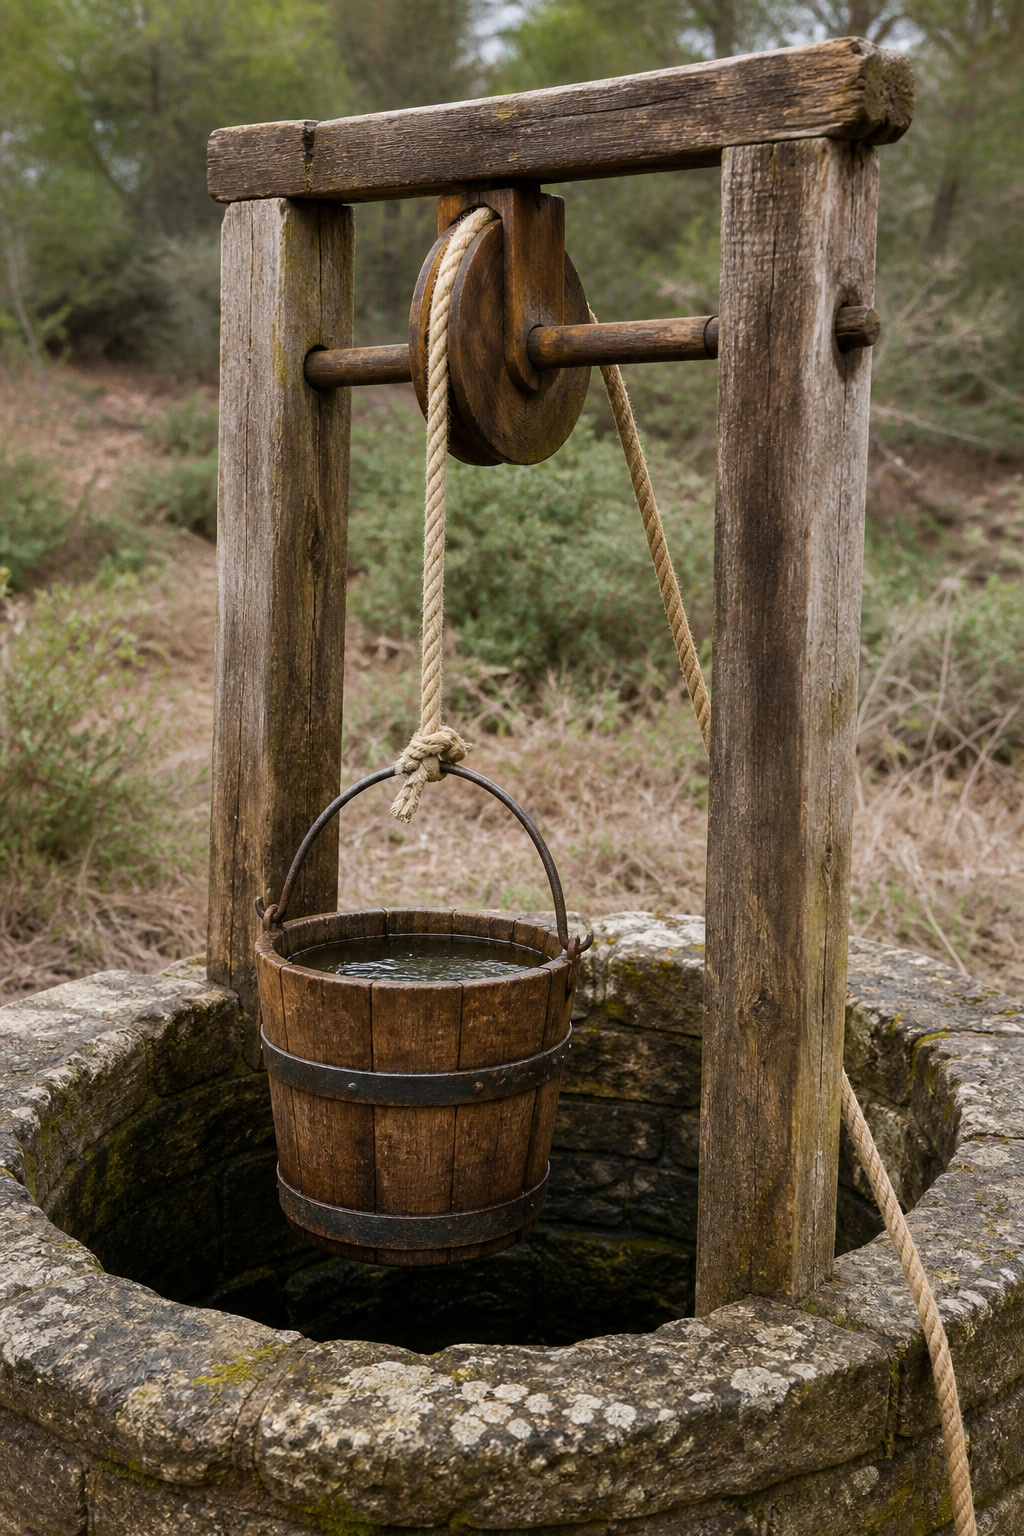
\includegraphics[width=0.34\linewidth]{images/book1/ai/g5-machines-pulley.jpg}

{\small The well's \omterm{def:g5:simple-machines:pulley}{pulley}: the rope rides in the groove, and a downward pull becomes an upward lift.}
\end{omfigure}

\begin{example}[Pulleys at work]\label{ex:g5:simple-machines:pulleywork}
The flag rises up its pole while your hands pull comfortably
\emph{down}: a fixed \omterm{def:g5:simple-machines:pulley}{pulley} at the top --- direction changed,
effort unchanged, but hauling down lets your own \omterm{def:g4:weight-and-mass:weight}{weight} help. The
builder's block-and-tackle chains several \omterm{def:g5:simple-machines:pulley}{pulleys} so the load hangs
from four or six strands: each strand carries a quarter or a sixth
of the \omterm{def:g4:weight-and-mass:weight}{weight}, and one worker raises a piano. Watch the worker,
though: \omterm{def:g2:measuring-length:units}{metre} after \omterm{def:g2:measuring-length:units}{metre} of rope races through their hands, while
the piano creeps upward slowly.
\end{example}

\section{The inclined plane}

\begin{definition}[Inclined plane]\label{def:g5:simple-machines:ramp}
An \emph{inclined plane}\index{inclined plane} --- a ramp --- is a
slope for raising loads without lifting them straight up. The
gentler the slope, the smaller the push needed to move the load
along it: rolling a barrel up a long, gentle ramp is easy; up a
short, steep one, brutal; straight up, impossible.
\end{definition}

\begin{method}[Feel it with the rubber-band scale]\label{met:g5:simple-machines:measure}
Your rubber-band scale from last year can taste the difference:
\begin{enumerate}
  \item load a toy car onto a plank and hook the rubber band to it;
  \item prop the plank as a gentle ramp onto a low book pile; drag
        the car slowly up by the band and note the stretch;
  \item prop the same plank much steeper, onto a chair seat, and
        drag again.
\end{enumerate}
The steep drag stretches the band far more: steeper slope, bigger
effort. Gentle slopes really are gentle --- your instrument says
so.
\end{method}

\begin{omfigure}
\begin{tikzpicture}[scale=0.8]
  \draw[thick] (0,0) -- (11.2,0);
  \draw[very thick, omDef] (0.3,0) -- (6.5,2.0);
  \draw[thick, fill=omMeth, fill opacity=0.4]
    (2.8,0.82) rectangle ++(0.8,0.55);
  \draw[-Stealth, thick, omThm] (3.75,1.35) -- (4.65,1.64);
  \node[above, font=\small, omThm] at (3.4,1.75) {small push};
  \draw[very thick, omDef] (8.2,0) -- (10.2,2.0);
  \draw[thick, fill=omMeth, fill opacity=0.4]
    (8.75,0.5) rectangle ++(0.8,0.55);
  \draw[-Stealth, very thick, omThm] (9.75,1.25) -- (10.55,2.05);
  \node[above, font=\small, omThm] at (9.3,1.9) {big push};
  \node[below, font=\small] at (3.4,-0.3)
    {long gentle ramp to the same height};
  \node[below, font=\small] at (9.3,-0.3) {short steep ramp};
\end{tikzpicture}

{\small Same crate, same height to gain: the long gentle ramp asks
a small push over a long road; the steep ramp, a big push over a
short one.}
\end{omfigure}

\begin{example}[Ramps in the landscape]\label{ex:g5:simple-machines:ramps}
Wheelchair ramps run long and shallow beside short staircases ---
gentleness on purpose. Mountain roads zigzag: rather than attack
the summit straight up, they wrap a long, gentle \omterm{def:g5:simple-machines:ramp}{inclined plane}
back and forth across the slope. And the screw is a ramp in
disguise --- a slope wrapped around a rod, so each easy turn of the
screwdriver sneaks the screw a tiny step deeper.
\end{example}

\section{The golden rule}

\begin{proposition}[The golden rule of machines]\label{prop:g5:simple-machines:golden}
No \omterm{def:g5:simple-machines:machine}{simple machine} gives something for nothing: whatever it saves in
\omterm{def:g2:pushes-and-pulls:force}{force}, it charges back in distance. Half the \omterm{def:g2:pushes-and-pulls:force}{force} --- twice the
rope hauled, or twice the road traveled; a tenth of the \omterm{def:g2:pushes-and-pulls:force}{force} ---
ten times the road. Machine after machine, the trade is exact:
comfort is bought with \omterm{def:g2:measuring-length:units}{metres}.
\end{proposition}

\begin{example}[Checking the rule]\label{ex:g5:simple-machines:check}
The movable \omterm{def:g5:simple-machines:pulley}{pulley}: your hand pulls with half the \omterm{def:g2:pushes-and-pulls:force}{force}, and to
raise the load \qty{1}{m} you haul in \qty{2}{m} of rope --- both
strands must shorten by a \omterm{def:g2:measuring-length:units}{metre}. The crowbar: your end sweeps a
long arc, the boulder barely stirs. The ramp: the crate reaches the
same height, but you pushed it along the whole slope. Every saving
paid for, precisely.
\end{example}

\begin{remark}[Why the rule cannot be cheated]\label{rem:g5:simple-machines:whygolden}
Hiding under the golden rule is our old friend from the \omterm{def:g5:everyday-energy:energy}{energy}
chapter: lifting a load to a height costs a fixed helping of
\omterm{def:g5:everyday-energy:energy}{energy}, and no arrangement of ropes and planks changes the price.
Machines only let you pay it in smaller coins --- more of them. A
small \omterm{def:g2:pushes-and-pulls:force}{force} over a long road hands over the same \omterm{def:g5:everyday-energy:energy}{energy} as a big
\omterm{def:g2:pushes-and-pulls:force}{force} over a short one. The forever-machines failed for this very
reason: the bill is always the bill.
\end{remark}

\section{Exercises}

\begin{exercise}[$\star$]\label{exo:g5:simple-machines:1}
Name the three classic \omterm{def:g5:simple-machines:machine}{simple machines}, and one everyday place each
is found.
\end{exercise}

\begin{exercise}[$\star$]\label{exo:g5:simple-machines:2}
What does a fixed \omterm{def:g5:simple-machines:pulley}{pulley} change about your pull? What does a
movable \omterm{def:g5:simple-machines:pulley}{pulley} change?
\end{exercise}

\begin{exercise}[$\star$]\label{exo:g5:simple-machines:3}
Why is hauling a flag \emph{down}ward to raise it more comfortable
than lifting the same \omterm{def:g4:weight-and-mass:weight}{weight} straight up, even though the effort is
the same size?
\end{exercise}

\begin{exercise}[$\star$]\label{exo:g5:simple-machines:4}
With one movable \omterm{def:g5:simple-machines:pulley}{pulley}, the load hangs from two strands. What
share of the \omterm{def:g4:weight-and-mass:weight}{weight} does your hand hold? To raise the load
\qty{3}{m}, how much rope must you haul?
\end{exercise}

\begin{exercise}[$\star$]\label{exo:g5:simple-machines:5}
In \cref{met:g5:simple-machines:measure}, which ramp stretches the
rubber band more? What pays for the gentler ramp's smaller
stretch?
\end{exercise}

\begin{exercise}[$\star$]\label{exo:g5:simple-machines:6}
Why do mountain roads zigzag instead of running straight up the
slope? Which \omterm{def:g5:simple-machines:machine}{simple machine} is the whole road?
\end{exercise}

\begin{exercise}[$\star$]\label{exo:g5:simple-machines:7}
State the golden rule of machines. A machine lets you pull with a
tenth of the \omterm{def:g2:pushes-and-pulls:force}{force} --- what does it charge you?
\end{exercise}

\begin{exercise}[$\star$]\label{exo:g5:simple-machines:8}
How is a screw an \omterm{def:g5:simple-machines:ramp}{inclined plane} in disguise? What plays the role
of the long gentle road?
\end{exercise}

\begin{exercise}[$\star\star$]\label{exo:g5:simple-machines:9}
A block-and-tackle hangs a piano from four strands. What fraction
of the piano's \omterm{def:g4:weight-and-mass:weight}{weight} does the worker's hand pull? To raise the
piano \qty{2}{m}, how many \omterm{def:g2:measuring-length:units}{metres} of rope pass through their
hands?
\end{exercise}

\begin{exercise}[$\star\star$]\label{exo:g5:simple-machines:10}
A loading ramp is \qty{6}{m} long and rises \qty{1}{m}; pushing a
crate up it takes a modest push. The impatient movers cut a new
ramp only \qty{3}{m} long to the same platform. Using the golden
rule, compare the new push with the old one --- and explain why
``half the road'' was no bargain.
\end{exercise}

\begin{exercise}[$\star\star$]\label{exo:g5:simple-machines:11}
An advertisement offers a \omterm{def:g5:simple-machines:pulley}{pulley} set ``so clever that you pull one
\omterm{def:g2:measuring-length:units}{metre} of rope with half the \omterm{def:g2:pushes-and-pulls:force}{force} --- and the load rises a full
\omterm{def:g2:measuring-length:units}{metre}''. Put the claim on trial before the golden rule and the
\omterm{def:g5:everyday-energy:energy}{energy} bill of \cref{rem:g5:simple-machines:whygolden}: could any
arrangement of wheels and ropes honor it?
\end{exercise}
